\documentclass[a4paper, titlepage, 10pt]{article}

\usepackage[left=3cm, right=3cm, top=4cm, bottom=4cm]{geometry}
\usepackage{utopia}
\renewcommand{\familydefault}{\rmdefault}
\usepackage{courier}

\usepackage[utf8]{inputenc}
\usepackage{color}
\usepackage{caption}
\usepackage{subcaption}
\usepackage{array}
\usepackage[hidelinks]{hyperref}
\usepackage{graphicx}
\usepackage[square,sort,comma,numbers]{natbib}
\usepackage{float}
\usepackage{newunicodechar}
\usepackage{booktabs}
\usepackage{adjustbox}
\usepackage{rotating}
\usepackage{colortbl}
\usepackage{multirow}
\usepackage[table]{xcolor}
\usepackage{makecell}
\usepackage{widetext}
\usepackage[normalem]{ulem}
\usepackage{listings}
\usepackage{amsmath}
\usepackage{amssymb}
\usepackage{amsthm}
\usepackage{fvextra}
\usepackage{float}
\usepackage[all,cmtip]{xy}
\usepackage{tikz}
\usetikzlibrary{arrows.meta,positioning}
\usepackage{xcolor}
\usepackage{xy}
\xyoption{frame}

% \captionsetup[figure]{hypcap=false}  % Disable hypcap for all figures



% Define Rust language for listings
\lstdefinelanguage{Rust}{
  keywords={
    self,pub,struct,enum,impl,fn,let,mut,move,match,if,else,for,in,while,loop,
    return,break,continue,where,type,trait,use,unsafe,extern,const,static,
    as,box,ref,Result,Option,Some,None,Ok,Err,Vec,String,
  },
  sensitive=true,
  comment=[l]{//},
  morecomment=[s]{/*}{*/},
  string=[b]",
  morestring=[b]',
}

% Better handling of verbatim blocks
\DefineVerbatimEnvironment{Verbatim}{Verbatim}{breaklines=true,fontsize=\small}

\definecolor{codegreen}{rgb}{0,0.6,0}
\definecolor{codegray}{rgb}{0.5,0.5,0.5}
\definecolor{backcolour}{rgb}{0.95,0.95,0.92}

\lstdefinestyle{mystyle}{
    backgroundcolor=\color{backcolour},
    commentstyle=\color{codegreen},
    keywordstyle=\color{magenta},
    numberstyle=\tiny\color{codegray},
    stringstyle=\color{codegreen},
    basicstyle=\ttfamily\footnotesize,
    breakatwhitespace=false,
    breaklines=true,
    keepspaces=true,
    numbers=left,
    numbersep=5pt,
    showspaces=false,
    showstringspaces=false,
    showtabs=false,
    tabsize=2,
    postbreak=\mbox{\textcolor{red}{$\hookrightarrow$}\space},
}

\lstset{style=mystyle}

\setlength{\parindent}{0pt}
\pagenumbering{arabic}

% Document Information
\newcommand{\projectTitle}{Infrastructure for Stateless Account Abstraction on Fuel}
\newcommand{\name}{}
\newcommand{\timeFrame}{February 2025}
\newcommand{\docType}{Specification}

\begin{document}

\begin{titlepage}
\begin{center}



\begin{figure}[h!]
    \centering
    
\includegraphics[width=.7\linewidth]{images/Zap_Logo_black+purple+transp_bkg.png}
\end{figure}
\vspace{1cm}

\LARGE{\textbf{\docType}}\\[0.7cm]

% \Huge{\projectTitle}
\Large{\projectTitle}

\vspace{1cm} 

\Large{\textbf{\name}} \\[3pt]
\Large{\textbf{\name}} \\[3pt]


\vspace{0.5cm}
\large{Date: \timeFrame} \\

\vspace{1cm}

% \large{\textbf{Supervisor}}\\
% \supervisor\\
% \vspace{0.5cm}
% \textbf{Advisor}\\
% \advisor\\
\end{center}
\end{titlepage}

\newpage
\thispagestyle{empty}  % No page number on this page

\begin{center}
    \Large\textbf{Version Information}
\end{center}
\vspace{1cm}


\begin{tabular}{p{4cm}p{2cm}p{6cm}}  % Specify three columns with widths
\textbf{Document Version:} & 1.2.0 & \\
\textbf{Release Date:} & February 2025 & \\
\textbf{ZapWallet version tag:} & v0.8.0 \\
zap-contracts branch: & \texttt{dev\_testing} & \\
commit: & \texttt{135a6c628e458dbde1aa804dd746bb90e50a97df} & \\
\textbf{Compatible with:} & \multicolumn{2}{l}{ % Span the next two columns
    \begin{minipage}[t]{8cm}
    • Sway v0.66.6 \\
    • Fuel-Core v0.40.0
    \end{minipage}
}
\end{tabular}



\vspace{2cm}

\begin{tabular}{ll}
\textbf{Version History} & \\
\hline
1.0.0 & Initial specification release for code tag v0.8.0 \\
1.1.0 & Adding sections for Modules 00, 01, for code tag v0.8.0 \\
1.2.0 & Adding sections for Modules 02,03,04,05,07, for code tag v0.8.0 \\
\end{tabular}

\vspace{2cm}

\textbf{Notes:}
\begin{itemize}
    \item This specification describes the ZapWallet implementation as of February 2025
    \item All version numbers follow semantic versioning (MAJOR.MINOR.PATCH)
\end{itemize}

\newpage

\section{Introduction}
\label{sec:introduction}

% The following specification is broken down into two parts. (1) The Predicate wallet, written in Sway, (2) The backend RPC-API and "executor". \\
The following specification is broken down into two parts. The Predicate wallet written in Sway and the backend JSON-RPC api commands. \\

\textbf{Predicate Wallet:}\

The predicate wallet is a stateless account abstraction wallet written in Sway. The "wallet" contains the logic to validate a
specific transaction types signed by the owner of the wallet. \\

\textbf{Backend:}\

The backend consists of an RPC endpoint that accepts \texttt{eth\_},\texttt{net\_} and \texttt{zap\_} namespace calls and a project
(that is required to build the RPC) called the "zap-executor", which builds and sends transactions to Fuels network, implements the interface
from an API call to the graph-ql port of fuel-core and any translation to evm spec data structures. \\
\section{Predicate Wallet}
\label{sec:predi_wal}

Zaps predicate wallet enables stateless account abstraction, by way of secp256k1 private keys ability to sign transactions
that spend UTXOs at the predicate wallet. The "owner" of the predicate wallet is also the owner of the public/private
key pair used to sign the any transaction(s) to the wallet itself. Thus account abstraction is obtained from the original public/private
key. \\




\subsection{Validation types}

There are currently two transaction types that can be supplied to the predicate wallet within the data structure \texttt{PValidation}. \\


\texttt{tx\_type}:

\begin{enumerate}
    \setcounter{enumi}{-1} % Set the counter to start at -1
    \item Initialization transaction.
    \item EVM signed transaction (Legacy, EIP-1559).
\end{enumerate}


The data struct \texttt{PValidation} is the only data that is passed into the main() function of the predicate wallet.


\begin{small}
\begin{verbatim}
    pub enum SuppliedData {
        InitData: Init,         // type (0)
        SignedData: Bytes,      // type (1)
    }

    struct PValidation {
        tx_type: u64,
        data: SuppliedData,
    }
\end{verbatim}
\end{small}


If the \texttt{tx\_type} is equal to zero (0), \texttt{PValidation} contains \texttt{InitData} within the \texttt{SuppliedData} struct.

\begin{small} % Adjust the font size here
\begin{verbatim}
    pub struct Init {
        signature_owner: B512,      // signature of the Assetid.
        key: b256,                  // the Key, for nt AssetId.
        wit_index: u64,             // witness index.
    }
\end{verbatim}
\end{small}

\texttt{Init} is a data struct containing the compact signature (\texttt{signature\_owner}) of the nonce token asset id that will
be minted by the nonce manager contract within the current transaction. The key (\texttt{key}) that was used to create the nonce
token asset id (see section \ref{sec:asset_id}) and the witness index (\texttt{wit\_index}) of the witness to the current transaction.\\


If the \texttt{tx\_type} is equal to one (1), \texttt{PValidation} contains \texttt{SignedData} which is of type Bytes. The Bytes
in this case is an RLP encoded EVM typed transaction.



% ----------------------------------------------------------------------------------------------
\subsubsection{Validation logic type 0}
\label{sec:asset_id}

The purpose of \texttt{tx\_type} = 0 is to provide the validation logic for a transaction that initializes the predicate wallet. This consists of calling
the nonce manager contract which mints "nonce token" assets and sends the mint amount - 1 to the predicate wallet. Once the predicate wallet contains some
amount of this asset type, and the nonce manager contract contains at least 1 (one) of these assets, the predicate wallet is considered initialized.\\

The \texttt{tx\_type} = 0 transaction type is necessary to mint "nonce token" assets, without nonce tokens of a specific asset\_id held as a UTXO at the predicate
wallet address, \texttt{tx\_type} = 1 transactions will not work. Within an EVM Legacy and EIP-1559 transaction the "nonce" field is populated with
the current transaction count for the account (EOA) making the transaction call. This number (the nonce) is incremented every time a
transaction is successfully included in a block on an EVM compatible chain. However when constructing a predicate wallet (abstracted account) there is
no concept built in to a transaction type that includes the facility to obtain a transaction count for a particular address or predicate root. Therefore,
for a predicate wallet to validate EVM style transactions, that are presented to the predicate as a simple byte stream, there must be a some mechanism by
which a transaction count (for the predicate wallet) can persist past the scope of a single transaction. Nonce tokens serve the purpose of keeping track
of the transaction count of a predicate wallet. For each
successful transaction (EVM style) the nonce token count is reduced by one. That is, for every transaction, the total amount of nonce tokens (held as
a UTXO) are included as an input to the transaction and the total amount - 1 is included as a transaction output to the same transaction. Thus
giving the transaction builder an easy mechanism to obtain the current transaction count (nonce) of a predicate wallet.\\



To calculate the nonce (token) AssetId of the following example is given taking the variables:


\begin{small}
    \begin{verbatim}

32 byte "the key" or sub_id,
0000000000000000000000000000000000000000000000000000000000000001

32 bytes padded evm address,
000000000000000000000000ff03ffd5d3e881c60a91eaa30c67d03aec025c49

32 bytes the NonceManager3's own ContractId, (beta-5)
c4442b787992c3afa14c0bfdec61b2921192e87494b226829c2d276ab855fc19


The AssetId is calculated by this by:
h1 = sha256("padded_evm_address":"key")
h2 = sha256("contractid":"h1")
AssetId = h2
\end{verbatim}
\end{small}


example:

\begin{small}
\begin{verbatim}

sha256(
000000000000000000000000ff03ffd5d3e881c60a91eaa30c67d03aec025c49,
0000000000000000000000000000000000000000000000000000000000000001)
=
\end{verbatim}
\end{small}

\begin{small}
\href{https://emn178.github.io/online-tools/sha256.html?input_type=hex&input=000000000000000000000000ff03ffd5d3e881c60a91eaa30c67d03aec025c490000000000000000000000000000000000000000000000000000000000000001&hmac_input_type=utf-8}{\texttt{8a1aa9c4f2b55e2991a44f390d27c12617b2a9b0e9d48546f06b709374f3dfd8}}\\
\end{small}

\begin{small}
    \begin{verbatim}
sha256(
c4442b787992c3afa14c0bfdec61b2921192e87494b226829c2d276ab855fc19,
8a1aa9c4f2b55e2991a44f390d27c12617b2a9b0e9d48546f06b709374f3dfd8)
=
\end{verbatim}
\end{small}

\begin{small}
\href{https://emn178.github.io/online-tools/sha256.html?input_type=hex&input=c4442b787992c3afa14c0bfdec61b2921192e87494b226829c2d276ab855fc198a1aa9c4f2b55e2991a44f390d27c12617b2a9b0e9d48546f06b709374f3dfd8&hmac_input_type=utf-8}{\texttt{280ffeb1249eeb3807bb24c2f5d9d71f438e81e6b67145c9a00a3ae76f7d3a5d}}\\
\end{small}

Nonce token AssetId that will be minted:
\begin{small}
    \begin{verbatim}
280ffeb1249eeb3807bb24c2f5d9d71f438e81e6b67145c9a00a3ae76f7d3a5d
\end{verbatim}
\end{small}


The following outlines the procedure to construct the InitData struct and build the initialization transaction that calls the Zap Nonce Manager
contract to mint nonce tokens.\\

1. To obtain the nonce token id a user can calculate it on "by-hand" by the above method, or, obtain by calling the above zap JSON-RPC method \texttt{zap\_get\_assetidKey1()} with the EVM address
of the owner.\\

2. The nonce token AssetId (32byte value) is Signed by the use via connected wallet (if using the Zap frontend App) or by an appropriate Ethereum library (like ethers-rs)
and sent back as hex encoded bytes to the rpc as a compact signature.\\

3. The zap JSON-RPC method \texttt{zap\_get\_initializationTxid()} is called with the signers EVM address and compact signature from (2) as a parameters.\\

4. The return value from (3) is the initialization transaction id. The user is then required to sign the 32-byte transaction id and return it the compact signature
to the zap rpc. The two options for this are 1; by the Zap frotnend using an EVM browser wallet extension that is connected, or, 2; with an appropriate
Ethereum library (like ethers-rs).\\

5. The zap JSON-RPC method \texttt{zap\_SubmitInitializationTx()} is called with two parameters, the compact signature from (4) and the EVM
signers address. This submits the initialization transaction to the Fuel node.\\

6. Once (5) is complete. transaction success can be checked by calling the eth JSON-RPC method \texttt{eth\_getTransactionReceipt()}.\\



% ----------------------------------------------------------------------------------------------
\subsubsection{Validation logic type 1}


The purpose of \texttt{tx\_type} = 1 is to provide the validation logic for a signed typed RLP encoded EVM transaction for the base asset (ETH) on Fuel.\\

The current predicate wallet supports Legacy and EIP-1559 EVM transactions. Both EVM transaction types are decoded by the predicate wallet itself and transaction
criteria are matched for validity.\\


\textbf{EVM Legacy Tx:} \\

The following example best explains how the \texttt{tx bytes rlp} from a Legacy EVM transaction are encoded and decoded within \texttt{rlp\_utls5.sw}.\\

transaction bytes encoded:\\
\begin{small}
    \begin{verbatim}
eb08822cb482520894ff03ffd5d3e881c60a91eaa30c67d03aec025c4987ea7aa
67b2d00008083097bc88080 + compact signature
    \end{verbatim}
\end{small}


\begin{small}
\begin{verbatim}
eb --> 0xc0 + length of payload (everything before the sig,
        not including the first byte ) 0xc0 + 0x2b = 0xeb
08 --> nonce
82 --> rlp encoded integer (0x80 and 0x02 bytes long)
2cb4 --> gas_price
82 --> rlp encoded integer (0x80 and 0x02 bytes long)
5208 --> gas_limit or max_fee_per_gas
94 --> rlp encoding
ff03ffd5d3e881c60a91eaa30c67d03aec025c49 --> to (evm address)
87 --> (0x80 and 0x07 bytes long)
ea7aa67b2d0000 --> value (amount wei)
8030
97bc8 --> chain_id --> odd number of characters
8080
\end{verbatim}
\end{small}


The logic for the above decoding can be seen in \texttt{rlp\_utls5.sw} from lines \href{https://github.com/Layer3Labs/zap-contracts/blob/9b2e0b8229077ef8becd6af0ad1a91f810a8db0a/contracts/wallet_predicate/src/rlp_utils5.sw#L153-L280}{\uline{153-280}}\\


\textbf{EVM EIP-1559 Tx:} \\

In a similar way the following example best explains how the \texttt{tx bytes rlp} from an EIP-1559 EVM transaction are encoded and decoded within \texttt{rlp\_utls5.sw}.\\

transaction bytes encoded:\\
\begin{small}
    \begin{verbatim}
02f87283097bc8018085011bd4e67982520894ff03ffd5d3e881c60a91eaa30c6
7d03aec025c49881148e7a6abbfc00080c001a0 + compact signature
    \end{verbatim}
\end{small}


\begin{small}
\begin{verbatim}
02 --> tx type
f872 --> rlp encoding byte length
83 --> rlp encoded 3 bytes
097bc --> chain id
80 --> rlp encoded 1 byte
1 --> nonce
8085 --> rlp encoded 5 bytes
011bd4e679 --> gas price
82 --> rlp encoded 2 bytes
5208 --> gas limit
94 --> rlp encoded 20 bytes
ff03ffd5d3e881c60a91eaa30c67d03aec025c49 --> to (evm address)
88 --> rlp encoding 8 bytes
1148e7a6abbfc000 --> value (wei)
80 --> rlp encoded 1 byte
c0
01a0 --> rlp encoded
\end{verbatim}
\end{small}

The logic for the above decoding can be seen in \texttt{rlp\_utls5.sw} from lines \href{https://github.com/Layer3Labs/zap-contracts/blob/9b2e0b8229077ef8becd6af0ad1a91f810a8db0a/contracts/wallet_predicate/src/rlp_utils5.sw#L72-L152}{\uline{72-152}}\\


\textbf{Tx validation:} \\

At the current \href{https://github.com/Layer3Labs/zap-contracts/commit/0e50f07c9350bb790d3a19d5302acd3ce96d310f}{\uline{commit}} a Legacy or EIP-1559 EVM transaction
is validated on the following conditions:\\

1. The transaction is signed by the owner of the predicate wallet (secp256k1 private key).\\
2. The transaction contains a nonce is equal to (0xFFFFFFFF - nonce) remaining nonce tokens held in the predicate wallet. \\
3. There is at least one one output for the remaining nonce tokens equal to (0xFFFFFFFF - (nonce -1 )) and returned to the predicate wallet.\\

Note: currently no checks are done against the value sent within the transaction or the change value. However, when the transaction is submitted to the RPC there
are change outputs added, and a failure will occur if the EVM signed transaction amount is greater than the predicate wallet balance.\



\newpage

\newpage
\section{Zap Manager Contract - {\ttfamily "ZapManager"}}
\label{sec:zapmanager_contract}


\subsection{Overview}
The ZapManager contract facilitates the initialization and upgrade lifecycle of a ZapWallet through asset management and state control. It serves as the central authority for:

\begin{itemize}
    \item Wallet initialization through controlled asset minting
    \item Upgrade path management between wallet versions
    \item State tracking through unique nonce assets
    \item Module asset distribution and verification
\end{itemize}

\subsection{State Variables}
The contract maintains the following state:

\begin{itemize}
    \item $owner \in Address$: Contract administrator with privileged access
    \item $v1\_map: key1 \rightarrow AssetId$: Nonce asset tracking where:
        \[ key1 = sha256(evm\_addr || master\_addr) \]
    \item $can\_initialize \in \{true, false\}$: Initialization phase flag
    \item $can\_upgrade \in \{true, false\}$: Upgrade phase flag
    \item $v1\_version, v2\_version \in String[5]$: Version identifiers
\end{itemize}

\subsection{Contract Phases}
Contract state evolves through distinct phases defined by the tuple $(can\_initialize, can\_upgrade)$ where:
\[ (can\_initialize, can\_upgrade) \in \{(false,false), (true,false), (false,true)\} \]

These phases represent:
\begin{itemize}
    \item $(false,false)$: Initial or paused state
    \item $(true,false)$: Active initialization phase
    \item $(false,true)$: Active upgrade phase
\end{itemize}

Phase transitions are controlled by the contract owner and must maintain the invariant:
\[ \neg(can\_initialize \land can\_upgrade) \]

\subsection{Core Functions}

\subsubsection{Wallet Initialization}
\begin{small}
\begin{verbatim}
initialize_wallet(master_addr, owner_evm_addr, initdata) -> EvmAddress
\end{verbatim}
\end{small}

\textbf{Preconditions:}
\begin{itemize}
    \item $\neg is\_paused()$
    \item $can\_initialize = true$ (for InitModules)
    \item $key1 \notin domain(v1\_map)$ (for InitModules)
\end{itemize}

\textbf{Effects:}
\begin{itemize}
    \item InitModules: Mints $(n+1)$ assets where $n = |modules|$ where:
        \[ \forall i \in [0,n]. balance(asset_i, recipient_i) = 1 \]
    \item NewModule: Mints single module asset where:
        \[ key \neq KEY\_NONCE \land balance(asset, recipient) = 1 \]
\end{itemize}

\textbf{Post-conditions:}
\begin{itemize}
    \item For InitModules:
        \[ key1 \in domain(v1\_map) \land balance(v1\_map[key1]) = 1 \]
    \item For NewModule:
        \[ balance(new\_module\_asset) = 1 \]
\end{itemize}






\subsubsection{Wallet Upgrade}
\begin{lstlisting}
upgrade(owner_evm_addr, sponsored)
\end{lstlisting}

\textbf{Preconditions:}
\begin{itemize}
    \item $\neg is\_paused()$
    \item $can\_upgrade = true$
    \item $\exists$ nonce asset in inputs where:
        \[ key1 = sha256(owner\_evm\_addr || nonce\_owner) \]
        \[ v1\_map[key1] = nonce\_asset\_id \]
\end{itemize}

\textbf{Effects:}
\begin{itemize}
    \item Verifies nonce asset ownership:
        \[ balance(nonce\_asset\_id, nonce\_owner) > 0 \]
    \item Records upgrade status
    \item Processes payment based on $sponsored$ flag
\end{itemize}

\subsection{Asset Management}
Asset balances and ownership are tracked through the balance function:
\[ balance: AssetId \times Address \rightarrow \mathbb{N} \]

Key generation for nonce asset tracking:
\[ key1 = sha256(evm\_addr || master) \]

Asset invariants must maintain:
\begin{itemize}
    \item Nonce uniqueness:
        \[ \forall k_1,k_2 \in domain(v1\_map). k_1 \neq k_2 \implies v1\_map[k_1] \neq v1\_map[k_2] \]
    \item Balance consistency:
        \[ \forall k \in domain(v1\_map). balance(v1\_map[k]) > 0 \]
\end{itemize}


% --------------------------------------------------------------------------------------------------
\subsection{Security Invariants}
% \begin{enumerate}
%     \item $\forall k. v1\_map[k] \neq \emptyset \implies balance(v1\_map[k]) > 0$
%     \item $\neg(can\_initialize \land can\_upgrade)$
%     \item $owner \neq \emptyset$
% \end{enumerate}

The security properties of the ZapManager contract are defined by the following formal invariants, which must hold true at all times during contract execution:

\subsubsection{Asset Mapping Integrity}
For any key in the nonce asset mapping:
\[ \forall k. v1\_map[k] \neq \emptyset \implies balance(v1\_map[k]) > 0 \]

This invariant ensures that any nonce asset recorded in the mapping must maintain a positive balance. This is critical for:
\begin{itemize}
   \item Preventing double initialization of wallets
   \item Maintaining unique wallet identities
   \item Ensuring valid upgrade paths
\end{itemize}

\subsubsection{Phase Exclusivity}
The contract phases must remain mutually exclusive:
\[ \neg(can\_initialize \land can\_upgrade) \]

This enforces strict separation between initialization and upgrade phases, which:
\begin{itemize}
   \item Prevents state confusion
   \item Ensures clean wallet lifecycle progression
   \item Maintains clear operational boundaries
\end{itemize}

\subsubsection{Administrative Control}
The contract must maintain valid ownership:
\[ owner \neq \emptyset \]

This invariant guarantees:
\begin{itemize}
   \item Continuous administrative control
   \item Emergency intervention capability
   \item Proper governance of contract parameters
\end{itemize}

\subsubsection{Asset State Consistency}
For any wallet $w$ with nonce asset $n$ and module assets $M$:
\[ balance(n) \in \{0, 1\} \]
\[ \forall m \in M. balance(m) \leq 1 \]

These balance constraints ensure:
\begin{itemize}
   \item Unique wallet identification through nonce assets
   \item Proper module asset distribution
   \item Prevention of asset duplication
\end{itemize}

\subsubsection{Verification}
These invariants are maintained through:
\begin{enumerate}
   \item Runtime checks in all state-modifying functions
   \item Access control restrictions on administrative operations
   \item Balance verification during initialization and upgrades
   \item Event emission for off-chain monitoring
\end{enumerate}

\subsubsection{Events}
Event emission follows state transitions:
\begin{itemize}
    \item InitializeWalletEvent(master\_addr, owner\_evm\_addr, is\_base\_modules)
    \item UpgradeEvent(owner\_evm\_addr, master\_address, is\_sponsored, verified\_nonce)
    \item ContractStateEvent(allow\_initialize, allow\_upgrade, sender)
    \item WalletVersionsEvent(v1\_version, v2\_version, sender)
\end{itemize}


\newpage
\section{Zap Master - {\ttfamily "master"}}
\label{sec:zapmaster_predicate}


\subsection{Overview}
The ZapWallet Master is a predicate that provides secure asset custody through modular validation. The master serves as the authority to validate
ZapWallet transactions, initialization (if paying own gas) and wallet upgrades.

\subsection{Definitions}

\textbf{Basic Types}\\
Let:
\begin{itemize}
    \item $\mathbb{B}_{256}$ be the set of 256-bit values
    \item $\mathbb{A}$ be the set of valid Fuel addresses
\end{itemize}

\textbf{Module}\\
A module $M$ is defined as a tuple:
\[ M = (a, p) \text{ where } a \in \mathbb{B}_{256}, p \in \mathbb{A} \]
where:
\begin{itemize}
    \item $a$ is the unique AssetId of the module
    \item $p$ is the predicate address of the module
\end{itemize}

\textbf{Wallet Configuration}\\
A wallet configuration $W$ consists of:
\[ W = (M_0, M_1, ..., M_8, o) \]
where:
\begin{itemize}
    \item $M_0$ is the upgrade module
    \item $M_1$ through $M_8$ are the operational modules
    \item $o \in \mathbb{B}_{256}$ is the owner's address
\end{itemize}




% ----------------------------------------------------------------------------------------------------
\subsection{Transaction Types and Validation}

The ZapWallet master predicate's \texttt{main()} function accepts an optional \texttt{WalletOp} parameter that serves two distinct purposes depending on the transaction type:

\begin{enumerate}
    \item \textbf{Initialization:} When present (\texttt{Some(WalletOp)}), validates wallet initialization
    \item \textbf{Module Operations:} When absent (\texttt{None}), validates module-based transactions
\end{enumerate}




\subsubsection{Initialization}
During initialization, \texttt{WalletOp} contains:

\begin{small}
\begin{verbatim}
pub struct WalletOp {
    pub evm_addr: b256,      // padded ETH address of wallet owner
    pub compsig: Bytes,      // Compact signature
    pub command: String,     // Initialization command
}
\end{verbatim}
\end{small}

An initialization transaction $T_i$ must satisfy:
\[ V_i(T_i, s, o) = true \]
where:
\begin{itemize}
    \item $s$ is a valid EIP712 signature
    \item $o$ is the owner's address
    \item $V_i$ is the initialization verification function
\end{itemize}

$V_i$ verifies:
\begin{enumerate}
    \item Exactly two inputs: one coin and one contract
    \item Valid change output
    \item Valid signature recovering to owner
    \item No module assets present
\end{enumerate}





\subsubsection{Module Operations}
For all other operations, transaction validation relies on:
\begin{itemize}
    \item Presence of exactly one module asset in inputs
    \item Proper return of module asset in outputs
    \item Module-specific validation logic
    \item Nonce token accounting (when required)
\end{itemize}

A module operation transaction $T_m$ must satisfy:
\[ V_m(T_m, M_i) = true \]
for exactly one module $M_i$ where $i \in \{1,...,8\}$

$V_m$ verifies:
\begin{enumerate}
    \item Exactly one module asset present in inputs
    \item Module asset returned correctly in outputs
    \item Module-specific validation passes
\end{enumerate}



\textbf{Upgrade Operation}\\
An upgrade transaction $T_u$ must satisfy:
\[ V_u(T_u, M_0) = true \]

$V_u$ verifies:
\begin{enumerate}
    \item Only module $M_0$ present
    \item Upgrade module asset handled correctly (sent to ZapManager)
    \item No other module assets present
\end{enumerate}



This dual-purpose design allows the \texttt{WalletOp} to handle initialization while remaining unintrusive for regular module operations.\\





\subsection{State Transitions}

\textbf{Module State Vector}\\
For any transaction T, let $\vec{m}$ be a boolean vector where:
\[ \vec{m} = [m_0, m_1, ..., m_8] \text{ where } m_i \in \{0,1\} \]
indicating the presence (1) or absence (0) of each module in the transaction inputs.\\

\textbf{Valid States}\\
A transaction is valid if and only if $\vec{m}$ satisfies exactly one of:
\begin{enumerate}
    \item Initialization: $\vec{m} = [0,0,...,0]$
    \item Single Module: $\vec{m}$ contains exactly one 1
    \item Upgrade: $\vec{m} = [1,0,...,0]$
\end{enumerate}



\subsection{Security Properties}

\textbf{Module Isolation}\\
For any valid transaction T:
\[ |\{i : m_i = 1\}| \leq 1 \]
Meaning no more than one module can be active in a single transaction.\\

\textbf{Asset Conservation}\\
For any module $M_i$ present in transaction inputs:
\[ \exists \text{ output } o : o.asset = M_i.a \land o.amount = 1 \land o.to = M_i.p \]
Meaning any module asset must be properly returned to its predicate.\\

\textbf{State Consistency}\\
The master predicate enforces:
\begin{itemize}
    \item No double-module usage
    \item Proper initialization sequence
    \item Upgrade isolation
    \item Module asset conservation
\end{itemize}


\subsubsection{Implementation Notes}

\textbf{Module Detection}\\
The system identifies modules by matching both:
\begin{itemize}
    \item AssetId ($\mathbb{B}_{256}$)
    \item Predicate Address ($\mathbb{A}$)
\end{itemize}

\textbf{Validation Flow}\\
1. Scan inputs for module assets
2. Build module state vector
3. Determine transaction type
4. Apply appropriate validation rules
5. Verify output conditions



% ---------------------------------------------------------------------------------------------------------------

\subsection{Initialization Flow}
The initialization of a ZapWallet can be done in one of two ways; using the owners Fuel \text{BASE\_ASSET} to pay for gas or from a third party that spends their own gas. If the owner is
initializing their own ZapWallet (self-initialization) this involves spending a \text{BASE\_ASSET} UTXO from the master, which requires a signature from the owner within
the \texttt{WalletOp} parameter of the master \text{main()} function call parameters. An initialization by way of a third party does not spend gas (or any other asset) from the
owners master.

\subsubsection{Self-Initialization}
A valid self-initialization initialization transaction requires:
\begin{itemize}
    \item Exactly two inputs:
        \begin{itemize}
            \item One coin input containing FUEL \text{BASE\_ASSET} for gas from the owners master address
            \item One contract input referencing the ZapManager contract
        \end{itemize}
    \item A single change output returning unused FUEL \text{BASE\_ASSET} to owners master address
\end{itemize}


The self-initialization route requires a single distinct signature from the owner. A standard EIP-712 compliant signature over the initialization data structure:
% \begin{small}
% \begin{verbatim}
% Initialization(
%     string command,    // "ZapWalletInitialize"
%     bytes32 evmaddr,   // Owner's padded EVM address
%     bytes32 utxoid     // UTXO ID of the gas coin input
% )
% \end{verbatim}
% \end{small}

\begin{lstlisting}
    Initialization(
        string command,    // "ZapWalletInitialize"
        bytes32 evmaddr,   // Owner's padded EVM address
        bytes32 utxoid     // UTXO ID of the gas coin input
    )
\end{lstlisting}


\subsubsection{Third Part Initialization}
A valid initialization transaction made my a third party requires:
\begin{itemize}
    \item Exactly two inputs:
        \begin{itemize}
            \item One coin input containing FUEL \text{BASE\_ASSET} for gas from whomever is sponsoring the transaction.
            \item One contract input referencing the ZapManager contract
        \end{itemize}
    \item A single change output returning unused FUEL \text{BASE\_ASSET} to the transaction sender
\end{itemize}







% --- calling the initialize_wallet() function at the ZapManager
\subsubsection{Contract Interaction}
The initialization flow proceeds as follows:
\begin{enumerate}
   \item The transaction calls the ZapManager contract function
    \begin{lstlisting}
    initialize_wallet()
    \end{lstlisting}

   \item The contract verifies no existing nonce token exists for the tuple $(a, m)$ where:
       \begin{itemize}
           \item $a \in \mathbb{B}_{256}$: The padded EVM address
           \item $m \in Address$: The master predicate address
       \end{itemize}
       See Section~\ref{subsec:overview-sec:zapmanager_contract} for details regarding the mapping.
   \item Upon verification, the contract:
       \begin{itemize}
           \item Mints the nonce tokens
           \item Sends (\text{NONCE\_MAX} - 1) to the ZapWallet master predicate
           \item Retains one token for transaction validation
       \end{itemize}
   \item The master predicate verifies:
       \begin{itemize}
           \item The initialization signature
           \item Transaction structure
           \item Change output validity
       \end{itemize}
\end{enumerate}




Upon successful completion of the \text{initialize\_wallet} function call, the ZapWallet is initialized and ready for module operations.


\newpage
\section{Module 00 - {\ttfamily "module00\_upgrade"}}
\label{sec:module00_predicate}

spec writeup WIP.


% The purpose of \texttt{tx\_type} = 0 is to provide the validation logic for a transaction that initializes the predicate wallet. This consists of calling
% the nonce manager contract which mints "nonce token" assets and sends the mint amount - 1 to the predicate wallet. Once the predicate wallet contains some
% amount of this asset type, and the nonce manager contract contains at least 1 (one) of these assets, the predicate wallet is considered initialized.\\

% The \texttt{tx\_type} = 0 transaction type is necessary to mint "nonce token" assets, without nonce tokens of a specific asset\_id held as a UTXO at the predicate
% wallet address, \texttt{tx\_type} = 1 transactions will not work. Within an EVM Legacy and EIP-1559 transaction the "nonce" field is populated with
% the current transaction count for the account (EOA) making the transaction call. This number (the nonce) is incremented every time a
% transaction is successfully included in a block on an EVM compatible chain. However when constructing a predicate wallet (abstracted account) there is
% no concept built in to a transaction type that includes the facility to obtain a transaction count for a particular address or predicate root. Therefore,
% for a predicate wallet to validate EVM style transactions, that are presented to the predicate as a simple byte stream, there must be a some mechanism by
% which a transaction count (for the predicate wallet) can persist past the scope of a single transaction. Nonce tokens serve the purpose of keeping track
% of the transaction count of a predicate wallet. For each
% successful transaction (EVM style) the nonce token count is reduced by one. That is, for every transaction, the total amount of nonce tokens (held as
% a UTXO) are included as an input to the transaction and the total amount - 1 is included as a transaction output to the same transaction. Thus
% giving the transaction builder an easy mechanism to obtain the current transaction count (nonce) of a predicate wallet.\\



\newpage
\section{Module 01 - {\ttfamily "module01\_evm\_txtype1"}}
\label{sec:module01_predicate}

% \subsection{Overview}
% Module 01 handles Legacy EVM transaction validation within the ZapWallet system. It validates and processes EVM transactions
% by decoding RLP-encoded transaction data, verifying signatures, and ensuring proper asset flow through the Fuel network. Module0 01
% only works for Fuel \text{BASE\_ASSET} transfers and the receiver should be the EVM address owner of a ZapWallet mapping.


\subsection{Overview}
Module 01 handles Legacy EVM transaction validation within the ZapWallet system. It validates and processes EVM transactions
by decoding RLP-encoded transaction data, verifying signatures, and ensuring proper asset flow through the Fuel network. Module 01
only works for Fuel \text{BASE\_ASSET} transfers. The receiver address in the RLP transaction data is an EVM address which maps
to a corresponding ZapWallet master predicate address. \\

Formally, for a transaction $T$ with recipient EVM address $r_{evm}$, the receiving ZapWallet address $w$ is derived:

\[ f: r_{evm} \rightarrow w \text{ where } w = P(r_{evm}, c) \]

where:
\begin{itemize}
   \item $P$ is the predicate address calculation function
   \item $c$ is the receiver's wallet bytecode
   \item $w$ is the resulting ZapWallet master predicate address
\end{itemize}

This mapping and calculation of the receivers address insures that EVM-style transactions are compatible with with ZapWallet's and
by extension the Fuel network, while maintaining proper asset custody.



% % ----------------------------------------------------------------------------------------------
% Merkle and address mapping

\subsection{Receiver Address Mapping}
For each transaction, Module 01 must verify that the Fuel \text{BASE\_ASSET} is sent to the correct ZapWallet address corresponding
to the EVM address specified in the RLP transaction data. This mapping is accomplished through a merkle tree-based predicate address calculation.

\subsubsection{Merkle Tree Structure}
The ZapWallet master predicate address is derived from a two-leaf merkle tree where:
\begin{itemize}
    \item Left Leaf ($L_1$): Fixed blueprint hash known at compilation
    \item Right Leaf ($L_2$): Variable leaf containing receiver's EVM address and configurables for the receiver's master predicate.
\end{itemize}

% The derivation process follows:
% \[ H(L_2) = \text{SHA256}(0 \parallel bytecode[EVM_{addr}]) \]
% \[ N = \text{SHA256}(1 \parallel L_1 \parallel H(L_2)) \]
% \[ root = N \]
% \[ address = \text{SHA256}(\texttt{FUEL} \parallel root) \]

% where:
% \begin{itemize}
%     \item $0$ is the leaf prefix byte
%     \item $1$ is the node prefix byte
%     \item $\texttt{FUEL}$ is the contract ID seed (\texttt{0x4655454C})
%     \item $EVM_{addr}$ is placed at position 6760 in the right leaf
% \end{itemize}

The derivation process follows these precise steps:

\textbf{1. Leaf Hashing:}
\[ H(L_2) = \text{SHA256}(\texttt{0x00} \parallel bytecode[EVM_{addr}]) \]
where \texttt{0x00} is the leaf prefix identifying this as a leaf node

\textbf{2. Node Computation:}
\[ N = \text{SHA256}(\texttt{0x01} \parallel L_1 \parallel H(L_2)) \]
where \texttt{0x01} is the node prefix identifying this as an internal node

\textbf{3. Root:}
\[ root = N \]

\textbf{4. Predicate Address:}
\[ address = \text{SHA256}(\texttt{0x4655454C} \parallel root) \]
where \texttt{0x4655454C} represents "FUEL" in ASCII as the contract ID seed. For a complete
implementation of Fuel's merkle tree specification, see the official implementation
at \url{https://github.com/FuelLabs/fuel-vm/tree/master/fuel-merkle}.


\subsubsection{Verification Process}
For a transaction with recipient EVM address $r_{evm}$, Module 01:
1. Takes the provided right leaf bytecode
2. Inserts $r_{evm}$ at the predetermined position (6760)
3. Calculates the merkle tree and resulting predicate address
4. Verifies the \text{BASE\_ASSET} output is sent to this address

This ensures that funds from EVM-style transactions are always directed to the correct ZapWallet predicate address,
maintaining the mapping between EVM addresses and their corresponding ZapWallets.






% % ----------------------------------------------------------------------------------------------
% RLP

\subsection{RLP Transaction Decoding}
\label{subsec:rlp_decoding}

EVM transactions are encoded using Recursive Length Prefix (RLP) encoding (previous to simple serialize (SSZ)). Modules 01-03 implement
RLP decoding systems for Legacy and EIP-1559 transactions (which can include ERC20 transfers). This RLP decoding scheme
is similar across Modules 01, 02 and 03 in the ZapWallet and can be broken down into several layers:

\subsubsection{RLP Encoding Rules}
The decoder follows standard Ethereum RLP encoding rules where bytes are categorized by their first byte (prefix):
\begin{itemize}
    \item \texttt{[0x00-0x7f]}: Single byte (transaction type identifier)
    \item \texttt{[0x80-0xb7]}: String with length 0-55 bytes
    \item \texttt{[0xb7-0xbf]}: String with length $>$ 55 bytes
    \item \texttt{[0xc0-0xf7]}: List with total payload 0-55 bytes
    \item \texttt{[0xf7-0xff]}: List with total payload $>$ 55 bytes
\end{itemize}


% -------------------------------------------------------------------------
% Legacy

\subsubsection{Legacy EVM Transaction Structure}
A Legacy EVM transaction's RLP encoding contains the following fields in order:
\begin{lstlisting}
[
    nonce,           // u64: Transaction sequence number
    gasPrice,        // u64: Price per unit of gas
    gasLimit,        // u64: Maximum gas allowed
    to,              // b256: Recipient address
    value,           // u256: Amount of ETH to transfer
    chainId,         // u64: Network identifier (EIP-155)
    r,               // b256: Signature component
    s                // b256: Signature component
]
\end{lstlisting}

\subsubsection{Decoding Process}
The decoding process follows these steps:

1. \textbf{Payload Identification}:
\begin{itemize}
    \item Reads the first byte to determine the encoding type
    \item Calculates total payload length
    \item Validates encoding structure
\end{itemize}

2. \textbf{Field Extraction}:
\[ decode: \text{RLP} \rightarrow (field, ptr, len) \]
where:
\begin{itemize}
    \item $field$ is the decoded value
    \item $ptr$ is the new buffer position
    \item $len$ is the field length
\end{itemize}

3. \textbf{Type Conversion}:
Different utilities handle specific data types:
\begin{itemize}
    \item \texttt{rlp\_read\_u64}: Converts bytes to unsigned 64-bit integer
    \item \texttt{rlp\_read\_b256}: Converts bytes to 256-bit value
    \item \texttt{rlp\_read\_bytes\_to\_u256}: Converts variable-length bytes to u256
\end{itemize}

\subsubsection{EIP-155 Processing}
The decoder implements EIP-155 chain ID recovery:
\[ chain\_id = \begin{cases}
    \frac{v - 35}{2} & \text{if } v \geq 35 \\
    0 & \text{otherwise}
\end{cases} \]

where $v$ is the recovery identifier from the signature.

\subsubsection{Signature Recovery}
The final step reconstructs the compact signature:
\begin{itemize}
    \item Normalizes the recovery ID
    \item Combines $r$ and $s$ components
    \item Sets the recovery bit in the high bit of $s$
\end{itemize}


% -------------------------------------------------------------------------
% EIP-1559

\subsubsection{EVM EIP-1559 Transaction Structure}
An EVM EIP-1559 (Type 2) transaction's RLP encoding contains the following fields in order:
\begin{lstlisting}
[
    chainId,              // u64: Network identifier
    nonce,               // u64: Transaction sequence number
    maxPriorityFeePerGas,// u64: Max priority fee (tip)
    maxFeePerGas,        // u64: Maximum total fee per gas
    gasLimit,            // u64: Maximum gas allowed
    to,                  // b256: Recipient address
    value,              // u256: Amount of ETH to transfer
    data,               // bytes: Transaction data (empty for simple transfers)
    accessList,         // []: List of addresses and storage keys
    v,                  // u64: Signature recovery identifier
    r,                  // b256: Signature component
    s                   // b256: Signature component
]
\end{lstlisting}


% -------------------------------------------------------------------------
% EIP-1559 ERC20

\subsubsection{EVM ERC20 Transaction Structure}
An EVM ERC20 transaction (Type 2) extends the EIP-1559 structure with specific data field encoding:
\begin{lstlisting}
[
    chainId,              // u64: Network identifier
    nonce,               // u64: Transaction sequence number
    maxPriorityFeePerGas,// u64: Max priority fee (tip)
    maxFeePerGas,        // u64: Maximum total fee per gas
    gasLimit,            // u64: Maximum gas allowed
    to,                  // b256: ERC20 contract address
    value,              // u256: Must be 0 for ERC20 transfers
    data: [             // bytes: Encoded transfer function call
        methodId,        // bytes4: transfer(address,uint256) selector
        recipient,       // b256: Token EVM recipient address
        amount          // b256: Amount of tokens to transfer
    ],
    accessList,         // []: List of addresses and storage keys
    v,                  // u64: Signature recovery identifier
    r,                  // b256: Signature component
    s                   // b256: Signature component
]
\end{lstlisting}

\textbf{ERC20 Data Field Details:}
The data field for ERC20 transfers consists of:
\begin{itemize}
    \item \texttt{methodId}: \texttt{0xa9059cbb} (transfer function selector)
    \item \texttt{recipient}: 32-byte padded address
    \item \texttt{amount}: 32-byte token amount
\end{itemize}

The field decoded to the ERC20 contract address is translated to the corresponding Fuel Native Asset ID
using the \texttt{compare\_asset\_ids} function. This allows Fuel native assets to be transferred as EVM ERC20 transfers on the Fuel network.



% % ----------------------------------------------------------------------------------------------
% % ----------------------------------------------------------------------------------------------
% Module 01 functionality


\subsection{Module 01 Core Functionality}
The module validates transactions through several key steps:
\begin{enumerate}
    \item RLP decoding of signed EVM transactions
    \item Signature and chain ID verification
    \item Asset input and output validation
    \item Nonce management
    \item Gas price and limit verification
\end{enumerate}

\subsection{Transaction Processing}
\subsubsection{EVM Transaction Decoding}
The module decodes Legacy EVM transactions into their constituent fields:
\begin{itemize}
    \item Chain ID (per EIP-155)
    \item Nonce
    \item Gas Price
    \item Gas Limit
    \item Recipient EVM Address
    \item Value (Base Asset amount in Wei)
    \item Signature Components (v, r, s)
\end{itemize}

\subsubsection{Validation Requirements}
For a transaction to be valid, it must satisfy:
\begin{itemize}
    \item Correct chain ID matching Fuel network
    \item Valid signature from wallet owner
    \item Sufficient input amounts covering value, gas and builder\_tip
    \item Proper nonce accounting matching the RLP data
    \item Valid input and output coins with correct owners
\end{itemize}


The builder\_tip needs be a Coin Output with some value (can be zero). It is not enforced that the transaction builder
is required to "tip" themselves. Therefore, the value of the \text{BASE\_ASSET} output to the receiver is always the amount specified in the RLP
data. The gas consumed by the transaction comes out of the \text{max\_tx\_cost} budget, which is made up of:

\[
\text{max\_tx\_cost} = \text{Fuel network fee} + \text{builder\_tip}
\]

Any difference in \text{BASE\_ASSET} that is not consumed by the sum of the transaction outputs (for \text{BASE\_ASSET}) is sent back to the
owners ZapWallet master Address as a Change output.


\subsection{Asset Flow}
A transaction containing Module 01 processes three types of assets:
\begin{itemize}
    \item Module 01 asset (for validation authorization of the signed RLP data)
    \item Nonce asset (to prevent signature replay)
    \item \text{BASE\_ASSET} (for value transfer and gas) from the master
\end{itemize}




\subsection{Transaction Structure}
\begin{figure}[H]
    \scalebox{0.85}{
    \centerline{
    \xymatrix@R=2.5pc@C=1.5pc{
        & \txt{Input type\\ Asset type\\ Amount}
        & \txt{Verification\\ Signature \\ type}
        & \txt{Output type\\ Receiver\\ Asset type\\ Amount} \\
        & *+[F]\txt{Coin predicate:\\ Module 01\\ asset: Module 01\\ AssetId\\ amount: 1}
            \ar[r] & *+[H]\txt{Legacy EVM\\ Transaction}
            \ar[r] & *+[F]\txt{type: Coin\\ to: Module 01\\ asset: Module 01\\ AssetId\\ amount: 1} \\
        & *+[F=]\txt{Coin predicate:\\ Master\\ asset: Nonce AssetId\\ amount: $n$,\\ where $n \geq 1$}
            \ar[r] & *+[H]\txt{Nonce value \\ \& ownership\\ validation}
            \ar[r] & *+[F=]\txt{type: Coin\\ to: Master\\ asset: Nonce AssetId\\ amount: $n - 1$} \\
        & *+[F=]\txt{Coin predicate:\\ Master\\ asset: BASE\_ASSET\\ amount:\\ value + max\_tx\_cost}
            \ar[r] & *+[H]\txt{Value \&\\ max\_tx\_cost \\ Validation}
            \ar[r] & *+[F=]\txt{type: Coin\\ to: Receiver\\ asset: BASE\_ASSET\\ amount: value} \\
        & \phantom{*+[F=]\txt{Placeholder}}
            \ar[r] & *+[H]\txt{max\_tx\_cost\\ Validation}
            \ar[r] & *+[F.:purple:dashed]\txt{type: Coin\\ to: Transaction\\ Builder\\ asset: BASE\_ASSET\\ amount:\\ $\text{max\_tx\_cost} - \text{network fee}$} \\
        & \phantom{*+[F=]\txt{Placeholder}}
            & \phantom{*+[F=]\txt{Placeholder}}
            & *+[F.:grey:dashed]\txt{type: Change\\ to: master\\ asset: BASE\_ASSET\\ amount: \\ $\text{receiver value} - \text{network fee} - \text{network fee}$}
    }}
    }
    \caption{Compact Module 01 Legacy EVM Transaction Flow and Verification}
    \label{fig:legacy-flow-xy-compact}
\end{figure}


\subsection{Security Properties}

\subsubsection{Asset Conservation}
For module01 asset $M_1$ and predicate address $P$:
\[ \exists \text{ output } o : o.asset = M_1 \land o.amount = 1 \land o.to = P \]

\subsubsection{Nonce Sequencing}
For nonce value $n$ and transaction nonce $t$:
\[ n = NONCE\_MAX - t \]
\[ \exists \text{ output } o : o.asset = N \land o.amount = n - 1 \]

\subsubsection{Value Transfer}
For transaction value $v$ and max cost $c$:
\[ \sum \text{inputs} \geq v + c \]
\[ \exists \text{ output } o : o.asset = BASE\_ASSET \land o.amount = v \land o.to = receiver \]


\subsection{Error Handling}
The module includes error handling that propagates errors to at maximum the \text{main()} scope. However as predicates
must return boolean results, all errors result in a \text{false} returned from the main execution.


\newpage
\section{Module 02 - {\ttfamily ""module02\_evm\_txtype2"}}
\label{sec:module02_predicate}

spec writeup WIP.


\newpage
\section{Module 03 - {\ttfamily ""module03\_erc20"}}
\label{sec:module03_predicate}

spec writeup WIP.


\newpage
\section{Module 04 - {\ttfamily "module04\_txidwit"}}
\label{sec:module04_predicate}

\subsection{Overview}
Module 04 provides a simplified transaction validation mechanism based purely on EIP-191 signature verification of the transaction ID.
Unlike other modules, it allows arbitrary transaction structures but explicitly forbids the use of the owners ZapWallet nonce assets, making it suitable
for flexible operations that don't require a nonce for replay protection as this is already inherited by the UTXO model.\\

\subsection{Signature Verification}
The module validates transactions through EIP-191 personal sign format:\\

\subsubsection{Message Construction}
For transaction ID $txid$, the signed message is constructed as:
\[ message = \text{EthereumSignedMessage prefix} \parallel txid \]

where the prefix is the hex-encoded string \texttt{"x19Ethereum Signed Message:"} + newline character and the number 32 for the amount
of bytes in the messsage (the transaction id), represented as:
\begin{verbatim}
0x19457468657265756d205369676e6564204d6573736167653a0a3332
\end{verbatim}

The module verifies:
\[ signer = ecrecover(signature, keccak256(message)) = owner \]


\begin{figure}[H]
    \scalebox{0.75}{
    \centering
    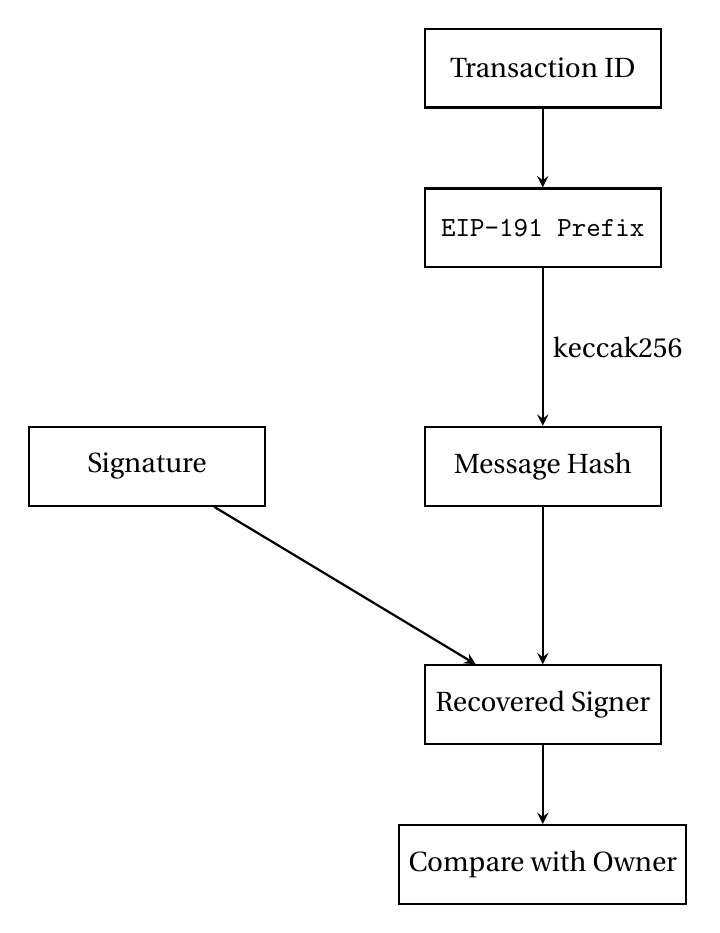
\begin{tikzpicture}[
        node distance=2cm,
        box/.style={rectangle, draw=black, thick, minimum width=3cm, minimum height=1cm, align=center},
        arrow/.style={-stealth, thick}
    ]
        % Transaction elements
        \node[box] (txid) {Transaction ID};
        \node[box] (prefix) [below=1cm of txid] {\texttt{EIP-191 Prefix}};
        \node[box] (hash) [below=2cm of prefix] {Message Hash};
        \node[box] (sig) [left=2cm of hash] {Signature};
        \node[box] (signer) [below=2cm of hash] {Recovered Signer};

        % Arrows
        \draw[arrow] (txid) -- (prefix);
        \draw[arrow] (prefix) -- node[right] {keccak256} (hash);
        \draw[arrow] (sig) -- (signer);
        \draw[arrow] (hash) -- (signer);

        % Validation result
        \node[box] (result) [below=1cm of signer] {Compare with Owner};
        \draw[arrow] (signer) -- (result);

    \end{tikzpicture}
    }
    \caption{Module 04 Signature Verification Flow}
    \label{fig:module04-flow}
\end{figure}







\subsection{Input Constraints}
While Module 04 is flexible in transaction structure, it enforces one critical constraint:\\

\[ \forall i \in inputs: i.assetId \neq NONCE\_ASSET\_ID \]

This ensures that:
\begin{itemize}
    \item Nonce-based replay protection remains under control of specific modules
    \item Blind Signature-based operations cannot interfere with nonce based Modules
\end{itemize}

\subsection{Usage Patterns}
Module 04 is designed for operations that need flexible input/output structures which can rely on transaction ID uniqueness
for replay protection. This can benefit transaction builders from simpler validation logic provided ZapWallet users are willing
to sign "blind" hashes.




\subsection{Security Properties}
Module 04 maintains two key security properties that ensure correct operation and prevent misuse:

\subsubsection{Signature Verification}
The module ensures that each transaction is properly authorized by the owner. For any transaction $T$ with witness signature $\sigma$:
\[ \exists \text{ witness } w : w = \sigma \land ecrecover(\sigma, hash(T)) = owner \]

This verifies that:
\begin{itemize}
   \item The transaction contains a valid witness signature
   \item The signature correctly recovers to the ZapWallet owner's address
   \item The signature was created over the exact transaction being processed
\end{itemize}

\subsubsection{Nonce Protection}
To maintain the integrity of the Nonce asset for use in other Modules, Module 04 explicitly forbids the use
of nonce assets. For all inputs $I$ in transaction $T$:
\[ \forall i \in I : i.asset \neq N \]
where $N$ is the nonce asset ID.\\

This constraint ensures that Nonce-based replay protection remains under the control of specific modules.


% \subsection{Security Properties}

% \subsubsection{Signature Verification}
% For transaction $T$ with witness signature $\sigma$:
% \[ \exists \text{ witness } w : w = \sigma \land ecrecover(\sigma, hash(T)) = owner \]

% \subsubsection{Nonce Protection}
% For all inputs $I$ in transaction $T$:
% \[ \forall i \in I : i.asset \neq N \]
% where $N$ is the nonce asset ID.
\newpage
\section{Module 05 - {\ttfamily ""module05\_eip712\_simple"}}
\label{sec:module05_predicate}

\subsection{Overview}
Module 05 is a native transfer predicate that handles both sponsored and unsponsored transactions for transferring \text{BASE\_ASSET} or other
native assets on the Fuel Network. It supports four types of transactions:\\

\begin{enumerate}
\item Non-Sponsored \text{BASE\_ASSET} transfer
\item Non-Sponsored other asset transfer
\item Sponsored \text{BASE\_ASSET} transfer
\item Sponsored other asset transfer
\end{enumerate}

Each transaction type has specific input and output requirements that must be met for the predicate to validate successfully. The predicate
checks the transaction structure, verifies the signature, and ensures proper asset flow according to the transaction type.




% % ----------------------------------------------------------------------------------------------
%

\subsection{Core Properties}
Module 05 implements a flexible native asset transfer system with properties that ensure secure asset movement and optional gas sponsorship.

\subsubsection{Transfer Properties}
For a transfer operation with value $v$, asset $a$, and owner $o$:
\[ \sum \{ i.amount : i \in inputs(a) | i.asset = a \land i.owner = o \} \]
\[ \exists \text{ unique output } o : o.asset = a \land o.amount = v \land o.to = recipient \]

\subsubsection{Sponsorship Properties}
For sponsored transactions with sponsor $s$ and asset $a$:
\[ s \neq owner\_wallet \]
\[ \begin{cases}
    \forall i \in inputs(BASE\_ASSET) : i.owner \in \{s, owner\} & a = BASE\_ASSET \\
    \forall i \in inputs(BASE\_ASSET) : i.owner = s & otherwise
\end{cases} \]


% % ---------------------------

\subsection{Signature Verification}
Module 05 uses EIP-712 typed data signing for transfer authorization. The \text{NativeTransfer} type hash is defined as:\\

\begin{lstlisting}
NativeTransfer(
   bytes32 Asset_Id,      // The Fuel native asset ID being transferred
   uint256 Amount,        // Amount of asset to transfer
   bytes32 From,          // Sender's ZapWallet master predicate address
   bytes32 To,            // Recipient's ZapWallet master predicate address
   uint256 Max_Tx_Cost,   // Maximum gas cost allowed for the transaction
   bytes32 Utxo_ID        // Transaction input ID of Module 05's asset
)
\end{lstlisting}

Each field serves a specific purpose in the transfer:
\begin{itemize}
   \item \texttt{Asset\_Id}: Identifies which Fuel native asset is being transferred, either \text{BASE\_ASSET} or another native asset
   \item \texttt{Amount}: Specifies the exact amount of the asset to transfer to the recipient
   \item \texttt{From}: The sender's ZapWallet master predicate address, which must match the transaction inputs
   \item \texttt{To}: The recipient's ZapWallet master predicate address where the assets will be sent
   \item \texttt{Max\_Tx\_Cost}: Sets a limit on transaction gas costs, protecting against excessive fees
   \item \texttt{Utxo\_ID}: The UTXO ID of Module 05's asset being consumed and returned in the transaction, preventing signature replay attacks
\end{itemize}

This structured data ensures the signed message unambiguously captures all aspects of the intended transfer, providing both
security and transparency.


% % ---------------------------

\subsection{Security Properties}
The module enforces three core security properties to ensure safe asset transfers:

\subsubsection{Asset Conservation}
The module ensures that its authorization token (Module 05 asset) is properly maintained:
\[ \exists \text{ output } o : o.asset = M_5 \land o.amount = 1 \land o.to = P \]

This means there must exist exactly one output that returns the Module 05 asset back to the module's predicate address,
maintaining the module's ability to validate future transactions.

\subsubsection{Amount Validation}
Verification that input amounts cover the requested transfer of amount $v$ of asset $a$ from owner $o$:
\[ \sum_{i \in I} i.amount \geq v \text{ where } i.asset = a \land i.owner = o \]


\subsubsection{Owner Authorization}
Every transfer must be authorized by the wallet owner through their signature:
\[ ecrecover(\sigma, hash(domain, m)) = owner \]




% % ----------------------------------------------------------------------------------------------
%
\subsection{Asset Flow}

The four types of transactions and their asset flow is shown below. \\


\subsubsection{Unsponsored \text{BASE\_ASSET} transfer}
For non-sponsored \text{BASE\_ASSET} transfers the inputs come exclusively from the owners ZapWallet master.\\


\textbf{Transaction Structure}:
\begin{figure}[H]
    \scalebox{0.85}{
    \centerline{
    \xymatrix@R=2.5pc@C=1.5pc{
        & \txt{Input type\\ Asset type\\ Amount}
        & \txt{Verification\\ Signature \\ Type}
        & \txt{Output type\\ Receiver\\ Asset type\\ Amount} \\
        & *+[F]\txt{Coin predicate:\\ Module 05\\ asset: Module 05\\ AssetId\\ amount: 1}
            \ar[r] & *+[H]\txt{EIP-712\\ Native Transfer}
            \ar[r] & *+[F]\txt{type: Coin\\ to: Module 05\\ asset: Module 05\\ AssetId\\ amount: 1} \\
        & *+[F=]\txt{Coin predicate:\\ Master\\ asset: BASE\_ASSET\\ amount: x}
            \ar[r] & *+[H]\txt{Transfer\\ Validation}
            \ar[r] & *+[F:blue]\txt{type: Coin\\ to: Receiver\\ asset: BASE\_ASSET\\ amount: $\text{value}$ } \\
        & \phantom{*+[F]\txt{Placeholder}}
            \ar[r] & *+[H]\txt{Asset \&\\ Amount\\ Validation}
            \ar[r] & *+[F=]\txt{type: Change\\ to: Master\\ asset: BASE\_ASSET\\ amount: $\text{remaining}$ } \\
        & \phantom{*+[F]\txt{Placeholder}}
            & \phantom{*+[H]\txt{Placeholder}}
            & *+[F]\txt{type: Coin\\ to: Master\\ asset: BASE\_ASSET\\ amount: $\text{GuaranteedChange}$ } \\
    }}
    }
    \caption{Unsponsored BASE\_ASSET Transfer Flow}
    \label{fig:module05-base-unsponsored}
\end{figure}




% % ----------------------------------------------------------------------------------------------
%
\newpage
\subsubsection{Unsponsored Native Asset Transfer}
For native asset transfers without sponsorship, both gas and the transferred asset come from the owners ZapWallet master.\\

\begin{figure}[H]
    \scalebox{0.85}{
    \centerline{
    \xymatrix@R=2.5pc@C=1.5pc{
        & \txt{Input type\\ Asset type\\ Amount}
        & \txt{Verification\\ Signature \\ Type}
        & \txt{Output type\\ Receiver\\ Asset type\\ Amount} \\
        & *+[F]\txt{Coin predicate:\\ Module 05\\ asset: Module 05\\ AssetId\\ amount: 1}
            \ar[r] & *+[H]\txt{EIP-712\\ Native Transfer}
            \ar[r] & *+[F]\txt{type: Coin\\ to: Module 05\\ asset: Module 05\\ AssetId\\ amount: 1} \\
        & *+[F=]\txt{Coin predicate:\\ Master\\ asset: BASE\_ASSET\\ amount: x}
            \ar[r] & *+[H]\txt{Gas\\ Validation}
            \ar[r] & *+[F=]\txt{type: Change\\ to: Master\\ asset: BASE\_ASSET\\ amount: remaining} \\
        & \phantom{*+[F]\txt{Placeholder}}
            & \phantom{*+[H]\txt{Placeholder}}
            & *+[F=]\txt{type: Coin\\ to: Master\\ asset: BASE\_ASSET\\ amount: GuaranteedChange} \\
        & *+[F=]\txt{Coin predicate:\\ Master\\ asset: Native Asset\\ amount: y}
            \ar[r] & *+[H]\txt{Asset \& Amount\\ Validation}
            \ar[r] & *+[F:blue]\txt{type: Coin\\ to: Receiver\\ asset: Native Asset\\ amount: value} \\
        & \phantom{*+[F]\txt{Placeholder}}
            & \phantom{*+[H]\txt{Placeholder}}
            & *+[F=]\txt{type: Change\\ to: Master\\ asset: Native Asset\\ amount: y - value}
    }}
    }
    \caption{Unsponsored Native Asset Transfer Flow}
    \label{fig:module05-native-unsponsored}
\end{figure}



% % ----------------------------------------------------------------------------------------------
%
\newpage
\subsubsection{Sponsored \text{BASE\_ASSET} Transfer}
In sponsored \text{BASE\_ASSET} transfers, a third party covers gas costs while the owners ZapWallet master provides the transfer amount.\\

\begin{figure}[H]
    \scalebox{0.85}{
    \centerline{
    \xymatrix@R=2.5pc@C=1.5pc{
        & \txt{Input type\\ Asset type\\ Amount}
        & \txt{Verification\\ Signature \\ Type}
        & \txt{Output type\\ Receiver\\ Asset type\\ Amount} \\
        & *+[F]\txt{Coin predicate:\\ Module 05\\ asset: Module 05\\ AssetId\\ amount: 1}
            \ar[r] & *+[H]\txt{EIP-712\\ Native Transfer}
            \ar[r] & *+[F]\txt{type: Coin\\ to: Module 05\\ asset: Module 05\\ AssetId\\ amount: 1} \\
        & *+[F:orange]\txt{Coin:\\ Sponsor\\ asset: BASE\_ASSET\\ amount: gas}
            \ar[r] & *+[H]\txt{Gas\\ Validation}
            \ar[r] & *+[F:orange]\txt{type: Change\\ to: Sponsor\\ asset: BASE\_ASSET\\ amount: remaining} \\
        & *+[F=]\txt{Coin predicate:\\ Master\\ asset: BASE\_ASSET\\ amount: x}
            \ar[r] & *+[H]\txt{Amount\\ Validation}
            \ar[r] & *+[F:blue]\txt{type: Coin\\ to: Receiver\\ asset: BASE\_ASSET\\ amount: value} \\
        & \phantom{*+[F]\txt{Placeholder}}
            & \phantom{*+[H]\txt{Placeholder}}
            & *+[F=]\txt{type: Change\\ to: Master\\ asset: BASE\_ASSET\\ amount: x - value}
    }}
    }
    \caption{Sponsored BASE\_ASSET Transfer Flow}
    \label{fig:module05-base-sponsored}
\end{figure}



% % ----------------------------------------------------------------------------------------------
%
\newpage
\subsubsection{Sponsored Native Asset Transfer}
Sponsored native asset transfers combine third-party gas coverage with native a asset from owners ZapWallet master. \\

\begin{figure}[H]
    \scalebox{0.85}{
    \centerline{
    \xymatrix@R=2.5pc@C=1.5pc{
        & \txt{Input type\\ Asset type\\ Amount}
        & \txt{Verification\\ Signature \\ Type}
        & \txt{Output type\\ Receiver\\ Asset type\\ Amount} \\
        & *+[F]\txt{Coin predicate:\\ Module 05\\ asset: Module 05\\ AssetId\\ amount: 1}
            \ar[r] & *+[H]\txt{EIP-712\\ Native Transfer}
            \ar[r] & *+[F]\txt{type: Coin\\ to: Module 05\\ asset: Module 05\\ AssetId\\ amount: 1} \\
        & *+[F:orange]\txt{Coin:\\ Sponsor\\ asset: BASE\_ASSET\\ amount: gas}
            \ar[r] & *+[H]\txt{Gas\\ Validation}
            \ar[r] & *+[F:orange]\txt{type: Change\\ to: Sponsor\\ asset: BASE\_ASSET\\ amount: remaining} \\
        & *+[F=]\txt{Coin predicate:\\ Master\\ asset: Native Asset\\ amount: y}
            \ar[r] & *+[H]\txt{Asset \& Amount\\ Validation}
            \ar[r] & *+[F:blue]\txt{type: Coin\\ to: Receiver\\ asset: Native Asset\\ amount: value} \\
        & \phantom{*+[F]\txt{Placeholder}}
            & \phantom{*+[H]\txt{Placeholder}}
            & *+[F=]\txt{type: Change\\ to: Master\\ asset: Native Asset\\ amount: y - value}
    }}
    }
    \caption{Sponsored Native Asset Transfer Flow}
    \label{fig:module05-native-sponsored}
\end{figure}
\newpage
\section{Module 06 - {\ttfamily ""module06\_eip712\_contract"}}
\label{sec:module06_predicate}

spec writeup WIP.


\newpage
\section{Module 07 - {\ttfamily ""module07\_sponsor"}}
\label{sec:module07_predicate}

\subsection{Overview}
Module 07 handles gas sponsorship operations from the owners ZapWallet. It validates and processes EIP-712 signed
gas sponsorship parameters, allowing gas UTXOs to be securely used for asset exchange, free usage, or sponsorship signatures
to be cancellation.\\


The module operates in three modes:
\begin{itemize}
\item \textbf{Sponsor}: Trade gas for another asset within configurable tolerance bounds
\item \textbf{Gaspass}: Allow free gas usage with guaranteed return amounts
\item \textbf{Cancel}: Move a gas UTXO without requiring exchange
\end{itemize}

% Formally, for a transaction $T$ with gas sponsorship operation $O$, the validation is:\\

% $[ v: O \rightarrow {true, false} \text{ where } O = (w, p) ]$ \\

Formally, for a transaction $T$ with gas sponsorship operation $O$, the validation is:

\begin{equation*}
v: O \rightarrow \{\text{true}, \text{false}\} \quad \text{where } O = (w, p)
\end{equation*}



where $v$ is the validation function, $O$ is the sponsorship operation tuple , $w$ is the EIP-712 signature
witness and $p$ are the sponsorship parameters\\


This allows gas UTXOs to be used flexibly and securely from the owners ZapWallet, enabling use cases like
transaction sponsorship, free trials, and cancellations while enforcing the sponsor's signed intent.\\

\subsection{Sponsorship Parameters}
The gas sponsorship parameters are defined by the \texttt{GasSponsor} struct:
\begin{lstlisting}
    struct GasSponsor {
    command: String,
    returnaddress: b256,
    inputgasutxoid: b256,
    expectedgasoutputamount: u256,
    expectedoutputasset: b256,
    expectedoutputamount: u256,
    tolerance: u256,
}
\end{lstlisting}

Where:
\begin{itemize}
\item \texttt{command}: Operation type (\texttt{"sponsor"}, \texttt{"gaspass"}, or \texttt{"cancel"})
\item \texttt{returnaddress}: Expected gas return address
\item \texttt{inputgasutxoid}: UTXO ID of the input gas coin
\item \texttt{expectedgasoutputamount}: Expected gas return amount
\item \texttt{expectedoutputasset}: Expected asset ID for exchange (\texttt{"sponsor"} only)
\item \texttt{expectedoutputamount}: Expected asset amount for exchange (\texttt{"sponsor"} only)
\item \texttt{tolerance}: Acceptable deviation from expected exchange amount (\texttt{"sponsor"} only)
\end{itemize}

These parameters are hashed according to EIP-712 and signed by the gas owner, providing secure authorization for the
specified usage of their gas UTXO.\\


\subsection{Validation Flow}
The core validation logic follows these steps:

\begin{enumerate}
\item Extract EIP-712 signature witness
\item Collect and categorize transaction inputs and outputs
\item Validate the specified gas UTXO is present and owned by signer
\item Process outputs according to \texttt{command}:
\begin{itemize}
\item \texttt{"sponsor"}: Verify asset exchange amounts are within tolerance
\item \texttt{"gaspass"}: Verify gas return amount
\item \texttt{"cancel"}: Validate gas UTXO movement
\end{itemize}
\item Rebuild \texttt{GasSponsor} struct and verify EIP-712 signature
\end{enumerate}

If all checks pass, the transaction is approved.\\



\subsection{Asset Flow}
A transaction containing Module 07 processes the following assets:

\begin{itemize}
\item \textbf{Gas UTXO}: The input gas coin (\text{BASE\_ASSET}) owned by the owners ZapWallet specified by \texttt{inputgasutxoid}
\item \textbf{Exchange Asset} (\texttt{"sponsor"} only): The asset traded to the gas owner
\end{itemize}

For the three different types of transactions \texttt{"sponsor"}, \texttt{"gaspass"} and \texttt{"cancel"} the asset flow is described below.\\


% % ----------------------------------------------------------------------------------------------
% sponsor
\subsubsection{\texttt{"sponsor"} Asset Flow}

The gas input UTXO must be present and owned by the owner of the ZapWallet. For \texttt{"sponsor"}
operations, the output exchange asset must match the \texttt{expectedoutputasset} and \\
\texttt{expectedoutputamount} and no \texttt{tolerance} is specified. Any remaining gas not explicitly output is returned
to the owner via a Change output.\\

\textbf{Transaction Structure}:
\begin{figure}[H]
    \scalebox{0.85}{
    \centerline{
    \xymatrix@R=2.5pc@C=1.5pc{
        & \txt{Input type\\ Asset type\\ Amount}
        & \txt{Verification\\ Signature \\ type}
        & \txt{Output type\\ Receiver\\ Asset type\\ Amount} \\
        & *+[F]\txt{Coin predicate:\\ Module 07\\ asset: Module 07\\ AssetId\\ amount: 1}
            \ar[r] & *+[H]\txt{Gas Sponsor\\ Validation}
            \ar[r] & *+[F=]\txt{type: Coin\\ to: Module 07\\ asset: Module 07\\ AssetId\\ amount: 1} \\
        & *+[F:purple]\txt{Coin:  User\\ asset: Other Coin AssetId\\ amount: $n$,\\ where $n \geq 1$}
            \ar[r] & *+[H]\txt{VM ownership validation \\ \& EIP712 Validation}
            \ar[r] & *+[F]\txt{type: Coin\\ to: Master\\ asset: Other Coin AssetId\\ amount: $\text{expectedoutputamount}$} \\
        & \phantom{*+[F=]\txt{Placeholder}}
            & \phantom{*+[F=]\txt{Placeholder}}
            \ar[r] & *+[F:purple]\txt{type: Change\\ to: User\\ asset: Other Coin AssetId\\ amount: $n - \text{expectedoutputamount}$} \\
        % ----------------------
        & *+[F=]\txt{Coin predicate: Master\\ asset: BASE\_ASSET\\ amount: value}
            \ar[r] & *+[H]\txt{Master Validation \&\\ EIP712 Validation}
            \ar[r] & *+[F=]\txt{type: Coin\\ to: Master\\ asset: BASE\_ASSET\\ amount: value - gas cost} \\
        & \phantom{*+[F=]\txt{Placeholder}}
            & \phantom{*+[F=]\txt{Placeholder}}
            \ar[r] & *+[F=]\txt{type: Change\\ to: Master\\ asset: BASE\_ASSET\\ amount: NA } \\
        % & \phantom{*+[F=]\txt{Placeholder}}
        %     & \phantom{*+[F=]\txt{Placeholder}}
        %     & *+[F.:grey:dashed]\txt{type: Change\\ to: master\\ asset: BASE\_ASSET\\ amount: \\ $\text{receiver value} - \text{network fee} - \text{network fee}$}
    }}
    }
    \caption{Module 07 Gas Sponsorship Transaction Flow for \texttt{"sponsor"}}
    \label{fig:module07-flow}
\end{figure}



% % ----------------------------------------------------------------------------------------------
% gasspass
\subsubsection{\texttt{"gasspass"} Asset Flow}

The gas input UTXO must be present and owned by the owner of the ZapWallet. For \texttt{"gasspass"}
operations, no exchange asset is required by the third party using the owners ZapWallet gas UTXO. The
\texttt{expectedgasoutputamount} gas return amount is specified by the owner. No \texttt{tolerance} is required. Any remaining gas not explicitly output is returned
to the owner via a Change output.\\




\textbf{Transaction Structure}:
\begin{figure}[H]
    \scalebox{0.85}{
    \centerline{
    \xymatrix@R=2.5pc@C=1.5pc{
        & \txt{Input type\\ Asset type\\ Amount}
        & \txt{Verification\\ Signature \\ type}
        & \txt{Output type\\ Receiver\\ Asset type\\ Amount} \\
        & *+[F]\txt{Coin predicate:\\ Module 07\\ asset: Module 07\\ AssetId\\ amount: 1}
            \ar[r] & *+[H]\txt{Gas Sponsor\\ Validation}
            \ar[r] & *+[F]\txt{type: Coin\\ to: Module 07\\ asset: Module 07\\ AssetId\\ amount: 1} \\
        % ----------------------
        & *+[F=]\txt{Coin predicate:\\ Master\\ asset: BASE\_ASSET\\ amount:\\ value}
            \ar[r] & *+[H]\txt{Master Validation \&\\ EIP712 Validation}
            \ar[r] & *+[F=]\txt{type: Coin\\ to: Master\\ asset: BASE\_ASSET\\ amount: $\text{expectedgasoutputamount}$} \\
        & \phantom{*+[F=]\txt{Placeholder}}
            & \phantom{*+[F=]\txt{Placeholder}}
            \ar[r] & *+[F=]\txt{type: Change\\ to: Master\\ asset: BASE\_ASSET\\ amount: NA } \\
        % & \phantom{*+[F=]\txt{Placeholder}}
        %     & \phantom{*+[F=]\txt{Placeholder}}
        %     & *+[F.:grey:dashed]\txt{type: Change\\ to: master\\ asset: BASE\_ASSET\\ amount: \\ $\text{receiver value} - \text{network fee} - \text{network fee}$}
    }}
    }
    \caption{Module 07 Gas Sponsorship Transaction Flow for \texttt{"gasspass"}}
    \label{fig:module07-flow}
\end{figure}


% % ----------------------------------------------------------------------------------------------
% cancel
\subsubsection{\texttt{"cancel"} Asset Flow}

For \texttt{"cancel"} operations, the UTXO of the owners gas is simply spent and sent back to the owner Zapwallet. This renders an already
signed \texttt{"sponsor"} or \texttt{"gasspass"} signature invalid. \\


\textbf{Transaction Structure}:
\begin{figure}[H]
    \scalebox{0.85}{
    \centerline{
    \xymatrix@R=2.5pc@C=1.5pc{
        & \txt{Input type\\ Asset type\\ Amount}
        & \txt{Verification\\ Signature \\ type}
        & \txt{Output type\\ Receiver\\ Asset type\\ Amount} \\
        & *+[F]\txt{Coin predicate:\\ Module 07\\ asset: Module 07\\ AssetId\\ amount: 1}
            \ar[r] & *+[H]\txt{Gas Sponsor\\ Validation}
            \ar[r] & *+[F]\txt{type: Coin\\ to: Module 07\\ asset: Module 07\\ AssetId\\ amount: 1} \\
        % ----------------------
        & *+[F=]\txt{Coin predicate:\\ Master\\ asset: BASE\_ASSET\\ amount:\\ value}
            \ar[r] & *+[H]\txt{Master Validation \&\\ EIP712 Validation}
            \ar[r] & *+[F=]\txt{type: Change\\ to: Master\\ asset: BASE\_ASSET\\ amount: NA} \\
    }}
    }
    \caption{Module 07 Gas Sponsorship Transaction Flow for \texttt{"cancel"}}
    \label{fig:module07-flow}
\end{figure}





% % ----------------------------------------------------------------------------------------------
%



\subsection{Security Properties}
\subsubsection{Signature Integrity}
The EIP-712 signature provides cryptographic verification of the gas sponsorship parameters through the
\texttt{GasSponsor} struct. The signing domain and struct type hash are fixed at deployment time, ensuring
immutability of the signature verification scheme.

The signature process follows:
\begin{equation*}
\begin{aligned}
\text{Signing}: & \quad s = \text{Sign}(H(\text{GasSponsor}), d_{\text{owner}}) \\
\text{Verification}: & \quad \text{Verify}(s, H(\text{GasSponsor}), d_{\text{contract}}) \rightarrow v
\end{aligned}
\end{equation*}

The components are defined as:
\begin{itemize}
\item $s$: Generated EIP-712 signature bytes
\item $H$: EIP-712 typed data hashing function
\item $d_{\text{owner}}$: Domain separator of the gas owner's signing context
\item $d_{\text{contract}}$: Domain separator of the verifying contract context
\item $v$: Boolean validation result of signature verification
\end{itemize}

This signature scheme ensures authenticity of owner intent, parameter integrity, cross-chain replay prevention, and verification
immutability through cryptographic signing, structured data hashing, domain separation, and fixed type hashes respectively.\\







\subsubsection{Asset Conservation}

The total output amounts are always equal to the input amounts, ensuring no assets are lost or created.
For a gas sponsorship transaction with gas amount $g$, expected return $r$, exchange amount $e$, and tolerance $t$:

\begin{equation*}
\begin{aligned}
\textbf{Sponsor Operation:} \\
\sum \text{outputs} &= \underbrace{(g - r)}_{\text{Unused gas}} + \underbrace{(e \pm t)}_{\text{Exchange asset}} + \underbrace{r}_{\text{Returned gas}} = g + (e \pm t) \\
\\
\textbf{Gaspass Operation:} \\
\sum \text{outputs} &= \underbrace{(g - r)}_{\text{Unused gas}} + \underbrace{r}_{\text{Returned gas}} = g \\
\\
\textbf{Cancel Operation:} \\
\sum \text{outputs} &= \underbrace{g}_{\text{Moved gas}}
\end{aligned}
\end{equation*}

In each case, the output amounts are conserved:
\begin{itemize}
\item \textbf{Sponsor}: The sum of unused gas, exchanged asset, and returned gas equals the input gas plus the exchange asset amount (within tolerance).
\item \textbf{Gaspass}: The sum of unused and returned gas equals the input gas amount.
\item \textbf{Cancel}: The output gas amount is equal to the input gas amount.
\end{itemize}

This asset conservation ensures that the gas sponsorship operations only move assets according to the validated parameters, without any loss or unauthorized creation of funds.\\







\subsubsection{Replay Prevention}
The \texttt{inputgasutxoid} parameter serves as a unique identifier for each gas sponsorship operation:

\begin{itemize}
\item \textbf{Uniqueness}: Each UTXO ID can only be used once
\item \textbf{Binding}: The ID is cryptographically bound to the signature
\item \textbf{Invalidation}: Once spent, the UTXO ID cannot be reused
\end{itemize}

This mechanism prevents transaction replay attacks, double-spending of gas UTXOs and reuse of sponsorship signatures. \\



\subsection{Error Handling}
The module includes error handling that propagates errors to at maximum the \text{main()} scope. However as predicates
must return boolean results, all errors result in a \text{false} returned from the main execution.




\newpage
\section{Module 08 - {\ttfamily ""module08"}}
\label{sec:module08_predicate}

Not implemented in v0.8.0 ZapWallet.



\clearpage
\bibliographystyle{plain}
{\small 
\bibliography{references}
}

\end{document}
